\subsection{Translinear Circuits}

\subsubsection{Short intro}

Before we start on explaining the translinear principle, let's touchbase on what translinear means altogether. Trans can mean a few different things in its Latin origin, but here, it means "going beyond". So translinear kinda means that we're going beyond linearity. But linearity of what? Linearity of current-voltage characteristic. Yes, our course is all about operating transistors in subthreshold and making them translinear: we have an exponential relationship between current and voltage, and not a linear one. That's it, that's what this fancy terms is all about. 

So a translinear circuit is a circuit that uses translinear circuit elements: MOSFETs operating in subthreshold (or BJT\footnote{Bipolar Junction Transistors (BJT) are another type of transistors which we don't really discuss in this course but are very popular in many applications.}) and hence in the exponential current voltage relation. 

\subsubsection{Translinear principle}

Static tranlinear circuits were invented by the late Barrie Gilbert, and there is actually a whole lecture on Youtube where he explains what this is all about \footnote{\url{https://www.youtube.com/watch?v=LQNJVtcFrCc}}. Let's write the formal definition: \textit{"In a closed loop containing an even number of forwardbiased junctions arranged so that there are an equal number of clockwise-facing and counter clock-wise facing polarities, the product of the current densities in the clockwise direction is equal to the product o the current densities in the counter clock-wise direction."}. This actually is best visualized by looking at a simple circuit (as opposed to the weird one shown in lecture notes):


\begin{figure}[H]
    \centering
    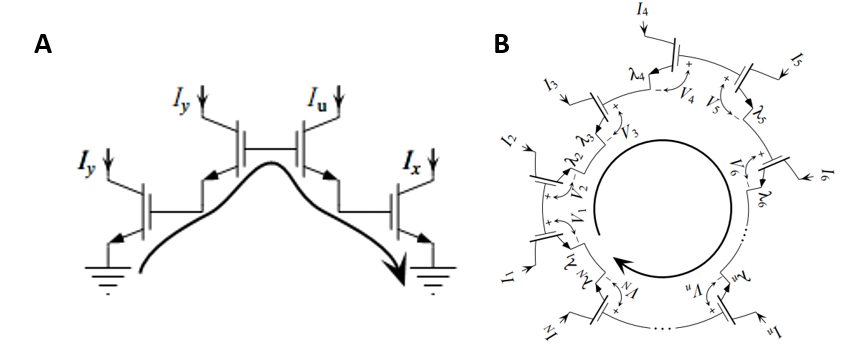
\includegraphics[width=0.8\linewidth]{../../Figures/Translinear_Principle.PNG}
    \caption{Two circuits with a translinear loop. A) Simple Translinear circuit. Adapted from Wikipedia. B) Complicated translinear circuit. Adapted from Lecture notes.}
    \label{fig:Translinear Principle}
\end{figure}

Consider figure \ref{fig:Translinear Principle}.A, you can see that there is an equal amount of clockwise facine and counter clockwise facing polarities BJTs \footnote{Yes, the images are shown with BJTs rather than MOSFETs. Don't worry too much about it.}. Remember Kirchoff's current law? (\textit{In any complete loop within a circuit, the sum of all voltages across components which supply electrical energy (such as cells or generators) must equal the sum of all voltages across the other components in the same loop.}). We can apply that to figure \ref{fig:Translinear Principle}.A (and B as well for the matter, and let's just focus on B because of the notation) and observe that the voltage around the loop that goes from $V_{1}$ to $V_{N}$ must be 0. In other words, the voltage drops must equal the voltage increases. We call this a translinear loop. Mathematically, this becomes

\begin{equation}
    \sum_{k=1}^{N} V_{F_K} = 0
\end{equation}

If you notice on the transistors, the $V_{F_K}$  on figure \ref{fig:Translinear Principle}.B are the gate to source voltages of the transistors. Imagining the image drew MOSFETS and not BJTs, that all transistors operate in saturation, and that $\kappa = 1$, we have each $V_{F_K} = U_T \mathrm{ln}(\frac{I_{ds_k}}{I_0})$. So now we can rewrite the previous sum as follows: 

\begin{equation}
    \sum_{k=1}^{N} {U_T \mathrm{ln}(\frac{I_{ds_k}}{I_0})} = 0
\end{equation}

We can exploit the logarithm property that $\mathrm{ln}(x \cdot y) = \mathrm{ln}(x) + \mathrm{ln}(y)$ and that ln$(1) = 0$  we reach the final: 

\begin{equation}
    \prod_{k=1}^{N} \frac{I_{DS_k}}{I_0} = 1
\end{equation}

The reason why this is useful will be visible soon enough. But mostly, if we have a circuit with a loop where sum of voltages is 0, we'll be able to apply this principle and we'll be happy.


